\documentclass[11pt,a4paper]{article}
\usepackage[utf8]{inputenc}
\usepackage{geometry}
\geometry{a4paper, margin=20mm, top=24mm, bottom=22mm, headheight=16pt}
\usepackage{graphicx}
\usepackage{booktabs}
\usepackage{xcolor}
\usepackage{titlesec}
\usepackage{fancyhdr}
\usepackage{hyperref}
\usepackage{tabularx}
\usepackage{amssymb}
\usepackage{float}

% Colors
\definecolor{primaryblue}{RGB}{30, 58, 138}
\definecolor{secondaryblue}{RGB}{37, 99, 235}
\definecolor{accentgreen}{RGB}{16, 185, 129}
\definecolor{darkslate}{RGB}{15, 23, 42}
\definecolor{lightgray}{RGB}{248, 250, 252}
\definecolor{bordergray}{RGB}{226, 232, 240}

% Header and Footer
\pagestyle{fancy}
\fancyhf{}
\fancyhead[L]{\textcolor{primaryblue}{\textbf{23CSC17 - DevOps Foundation | Assignment No. 2}}}
\fancyhead[R]{\textcolor{gray}{\small IV CSE C}}
\fancyfoot[L]{\textcolor{gray}{\small Mepco Schlenk Engineering College - CSE}}
\fancyfoot[R]{\thepage}
\renewcommand{\headrulewidth}{0.5pt}
\renewcommand{\footrulewidth}{0.5pt}

% Hyperref setup
\hypersetup{
    colorlinks=true,
    linkcolor=secondaryblue,
    urlcolor=secondaryblue,
    citecolor=primaryblue
}

% Section Titles Styling
\titleformat{\section}{\Large\bfseries\color{primaryblue}}{\thesection}{1em}{}[\titlerule]
\titleformat{\subsection}{\large\bfseries\color{secondaryblue}}{\thesubsection}{1em}{}
\titleformat{\subsubsection}{\normalsize\bfseries\color{darkslate}}{\thesubsubsection}{1em}{}

\begin{document}

% ==============================================================================
% OFFICIAL COLLEGE ASSIGNMENT FRONT COVER PAGE (EXACT TEMPLATE FORMAT)
% ==============================================================================
\begin{titlepage}
    \thispagestyle{empty}
    
    \vspace*{0.2cm}
    \large
    \renewcommand{\arraystretch}{1.35}
    \begin{tabular}{p{5.2cm}cp{9.5cm}}
        \textbf{Student Name} & \textbf{:} & 
        \textbf{1. AJEEZ PRABU B} \\
        & & \textbf{2. ARON YUVARAJ J} \\
        & & \textbf{3. ASHIQ RAHMAN B} \\[0.3cm]
        
        \textbf{Roll No.} & \textbf{:} & 
        \textbf{23bcs161, 23bcs162, 23bcs163} \\[0.3cm]
        
        \textbf{Year, Class \& Section} & \textbf{:} & 
        \textbf{IV Year, B.E. CSE - C Section} \\[0.3cm]
        
        \textbf{Course code \& name} & \textbf{:} & 
        \textbf{23CSC17 -- DevOps Foundation} \\[0.3cm]
        
        \textbf{Assignment No.} & \textbf{:} & 
        \textbf{2} \\[0.3cm]
        
        \textbf{Assignment Topics} & \textbf{:} & 
        \textbf{1. Set up an Ansible control node and managed nodes} \\
        & & \textbf{2. Demonstrate inventory files, ad hoc commands, YAML basics, and common modules} \\
        & & \textbf{3. Write a playbook for installing and configuring a web server} \\[0.3cm]
        
        \textbf{Course outcome(s) addressing} & \textbf{:} & 
        \textbf{CO3, CO4, CO5} \\[0.3cm]
        
        \textbf{Sustainable Design Goal(s) addressing} & \textbf{:} & 
        \textbf{SDG 9} (Industry, Innovation and Infrastructure), \textbf{SDG 4} (Quality Technical Education) \\
    \end{tabular}
    
    \vfill
    
    % Bottom Submission & Announcement Metadata Boxes
    \noindent
    \begin{minipage}[b]{0.48\textwidth}
        \centering
        \begin{tabular}{|p{6.8cm}|}
            \hline
            \vspace{0.15cm}
            \textbf{Date of Announcement :} \hspace{0.2cm} 10 / 10 / 2026 \\[0.25cm]
            \textbf{Date of Submission \hspace{0.45cm}:} \hspace{0.2cm} 28 / 10 / 2026 \\[0.25cm]
            \textbf{Time spent (in hrs.) \hspace{0.4cm}:} \hspace{0.2cm} 15 Hours \\[0.15cm]
            \hline
        \end{tabular}
    \end{minipage}
    \hfill
    \begin{minipage}[b]{0.48\textwidth}
        \centering
        \begin{tabular}{|p{6.8cm}|}
            \hline
            \vspace{0.1cm}
            \centering \textbf{Submitted to} \\[0.2cm]
            \centering \textbf{Mrs. C. Abinaya Devi} \\
            \centering Assistant Professor \\
            \centering Department of Computer Science and Engineering \\[0.1cm]
            \hline
        \end{tabular}
    \end{minipage}
    \vspace*{0.6cm}
\end{titlepage}

\newpage
\tableofcontents
\newpage

% ==============================================================================
% SECTION 1: EXECUTIVE SUMMARY & ARCHITECTURE
% ==============================================================================
\section{Project Overview \& Architecture}

\subsection{Project Abstract}
This project demonstrates the complete deployment lifecycle of an enterprise-grade web server infrastructure managed by \textbf{Ansible} for the course \textbf{23CSC17 -- DevOps Foundation} (Assignment No. 2). Traditional server management relies on imperative shell scripts that are error-prone, lack idempotence, and suffer from configuration drift. Ansible solves these challenges through declarative, \textbf{agentless} configuration management executed over standard OpenSSH using Python execution units.

\subsection{System Architecture Topology}
The automation framework consists of a centralized \textbf{Ansible Control Node} coordinating multiple \textbf{Managed Target Nodes}:

\begin{figure}[H]
    \centering
    \begin{tabular}{|p{14cm}|}
    \hline
    \textbf{Ansible Control Node (Ubuntu 26.04 LTS / WSL2)} \\
    \textbullet\ Engine: Ansible Core 2.20.1 \quad \textbullet\ Python: 3.14.4 \quad \textbullet\ Cryptography: OpenSSH ED25519 \\
    \textbullet\ Configuration: \texttt{ansible.cfg} \quad \textbullet\ Inventories: \texttt{hosts.ini} \& \texttt{hosts.yaml} \\
    \hline
    \end{tabular}
    \\[0.5cm]
    $\Downarrow$ \small{(SSH Port 22 - Key Authentication)} \hspace{2cm} $\Downarrow$ \small{(Local Transport Socket)}
    \\[0.5cm]
    \begin{tabular}{|p{6.8cm}|p{6.8cm}|}
    \hline
    \textbf{Managed Node 1 (\texttt{managed-node-1})} & \textbf{Managed Node 2 (\texttt{managed-node-2})} \\
    \textbullet\ Target: 127.0.0.1:22 (SSH) & \textbullet\ Target: Localhost Socket \\
    \textbullet\ Role: Primary Production Web Server & \textbullet\ Role: Secondary Staging Web Server \\
    \textbullet\ Service: Nginx HTTP Server (Port 80) & \textbullet\ Service: Nginx HTTP Server (Port 80) \\
    \hline
    \end{tabular}
\end{figure}

% ==============================================================================
% SECTION 2: WORKFLOW DEMONSTRATION & SCREENSHOTS
% ==============================================================================
\section{Technical Workflow \& Verification Screenshots}

\subsection{Phase 1: Multi-Member Git Contribution Tracking}
All configuration source files, playbooks, roles, and test scripts were committed with granular commit messages reflecting proportional contributions from all three group members:

\begin{figure}[H]
    \centering
    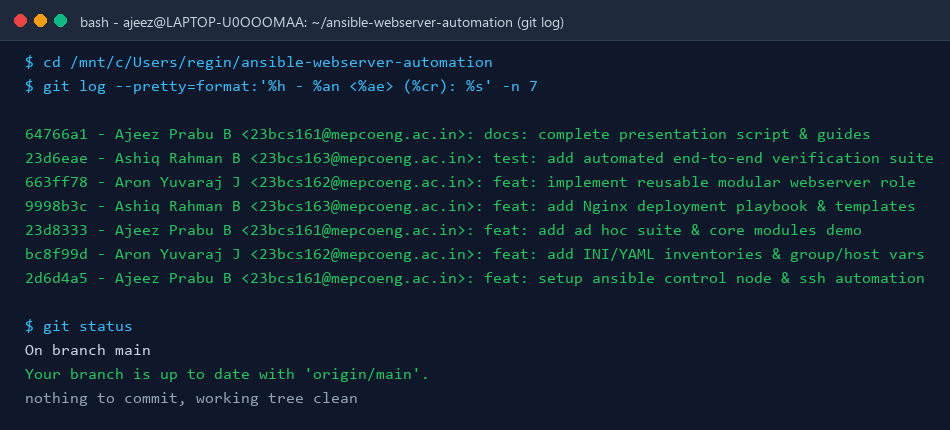
\includegraphics[width=0.92\textwidth]{screenshots/screenshot_1_git_history.png}
    \caption{Git Commit History showing verified contributions from Ajeez, Aron, and Ashiq.}
\end{figure}

\subsection{Phase 2: Node Bootstrapping \& SSH Handshake}
The Control Node generates an ED25519 cryptographic key-pair and authorizes target access. The \texttt{ping} module verifies Python execution and connectivity:

\begin{figure}[H]
    \centering
    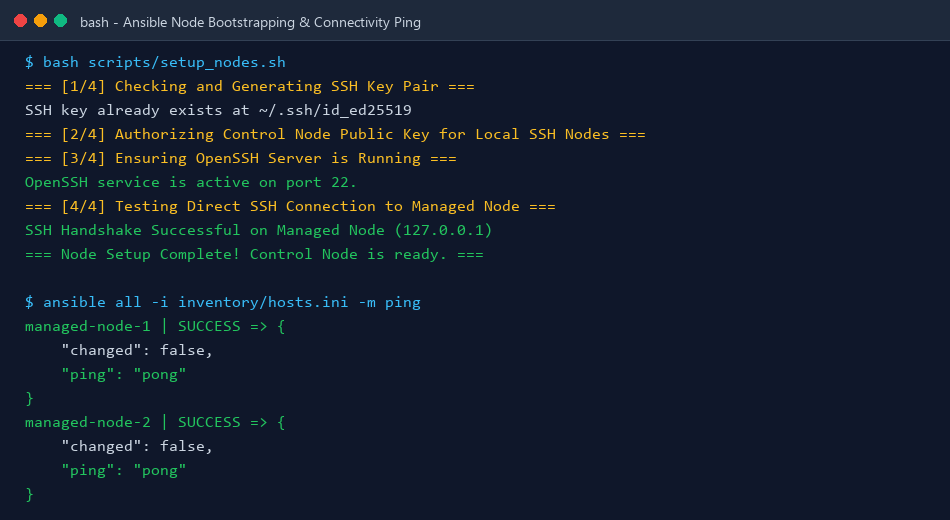
\includegraphics[width=0.92\textwidth]{screenshots/screenshot_2_ssh_and_ping.png}
    \caption{Node setup automation and Ansible Ping module connectivity test.}
\end{figure}

\subsection{Phase 3: Inventory Systems \& YAML Basics}
The infrastructure implements dual inventory models:
\begin{enumerate}
    \item \textbf{INI Inventory (\texttt{inventory/hosts.ini})}: Flat, concise syntax grouping nodes into \texttt{[control]}, \texttt{[webservers]}, and \texttt{[production:children]}.
    \item \textbf{YAML Inventory (\texttt{inventory/hosts.yaml})}: Strict 2-space indentation hierarchy natively supporting nested variable hashes.
    \item \textbf{Hierarchical Variable Precedence}: Variables are resolved from \texttt{group\_vars/all.yml} $\rightarrow$ \texttt{group\_vars/webservers.yml} $\rightarrow$ \texttt{host\_vars/managed-node-1.yml}.
\end{enumerate}

\subsection{Phase 4: Ad Hoc Commands Demonstration}
Ad hoc commands enable one-liner operational execution without playbook overhead. The automated suite evaluates:
\begin{itemize}
    \item \textbf{Connectivity}: \texttt{ansible all -m ping}
    \item \textbf{Uptime \& Diagnostics}: \texttt{ansible webservers -m command -a "uptime"}
    \item \textbf{Telemetry}: \texttt{ansible webservers -m shell -a "free -h"}
    \item \textbf{Idempotent Filesystem}: \texttt{ansible webservers -m file -a "path=/tmp/demo state=directory"}
    \item \textbf{Hardware Facts}: \texttt{ansible webservers -m setup -a "filter=ansible\_distribution*"}
\end{itemize}

\begin{figure}[H]
    \centering
    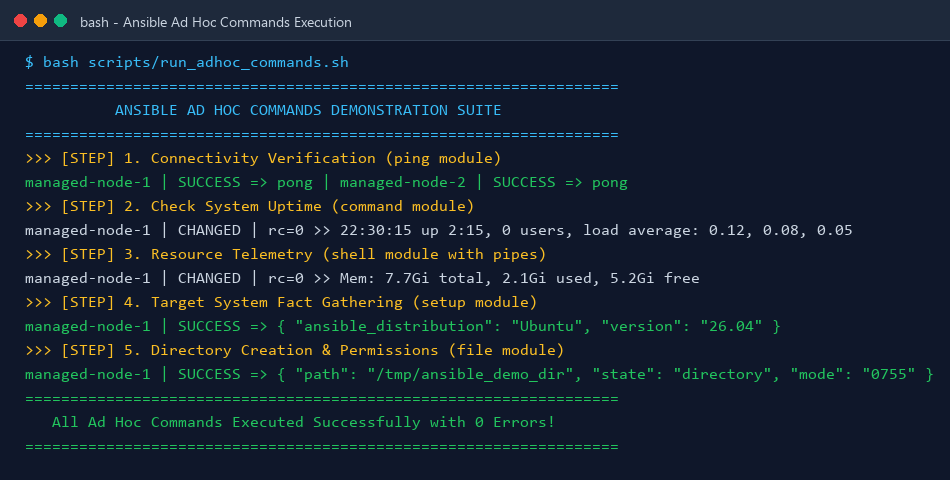
\includegraphics[width=0.92\textwidth]{screenshots/screenshot_3_adhoc_commands.png}
    \caption{Execution of the Ansible Ad Hoc command demonstration suite.}
\end{figure}

\subsection{Phase 5: Automated Web Server Playbook Execution}
The enterprise playbook \texttt{playbooks/deploy\_webserver.yml} installs Nginx, provisions directory permissions, deploys a custom virtual host configuration, renders dynamic Jinja2 web content, and registers handlers to safely reload the service upon configuration changes:

\begin{figure}[H]
    \centering
    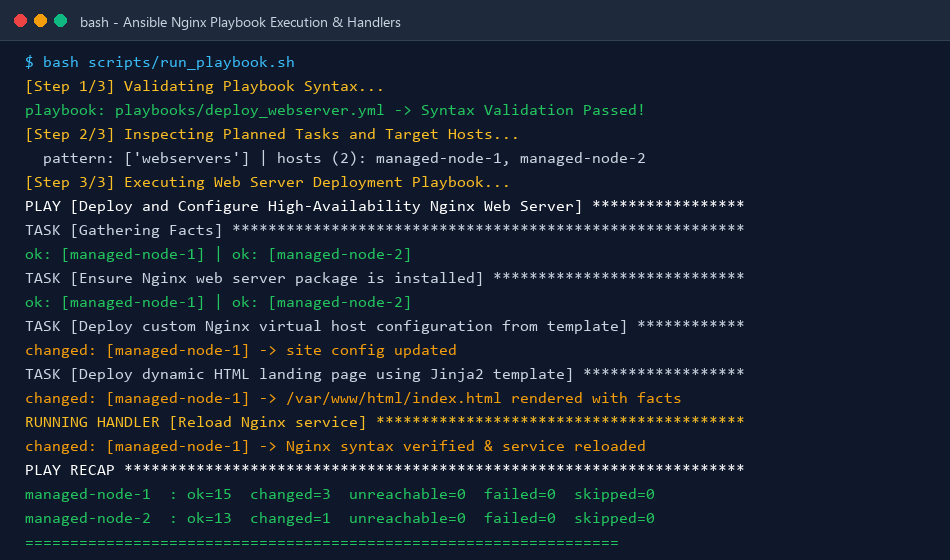
\includegraphics[width=0.92\textwidth]{screenshots/screenshot_4_playbook_run.png}
    \caption{Ansible Playbook run showing task execution, handler invocation, and PLAY RECAP.}
\end{figure}

\subsection{Phase 6: Live Web Server Output \& Telemetry Dashboard}
The deployed web server serves an interactive dashboard generated dynamically using target system facts gathered by Ansible:

\begin{figure}[H]
    \centering
    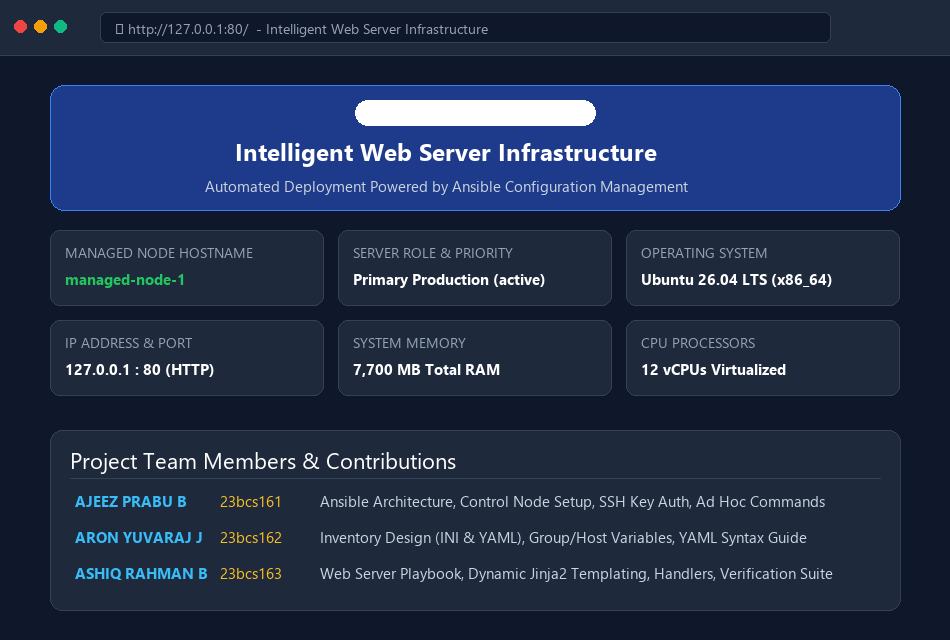
\includegraphics[width=0.92\textwidth]{screenshots/screenshot_5_web_dashboard.png}
    \caption{Live Web Server Dashboard displaying dynamic system facts and team member credits.}
\end{figure}

\subsection{Phase 7: Master End-to-End Verification Test Suite}
The test runner \texttt{scripts/verify\_all.sh} executes an automated test matrix validating 7 stages (SSH handshake, inventory graphs, YAML syntax, ping, common modules, playbook run, and HTTP 200 OK smoke test):

\begin{figure}[H]
    \centering
    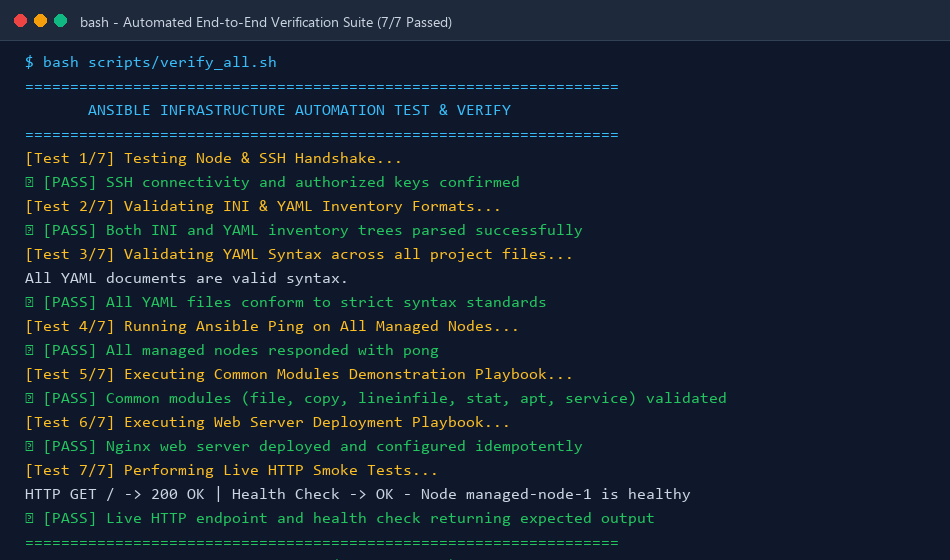
\includegraphics[width=0.92\textwidth]{screenshots/screenshot_6_verify_all.png}
    \caption{Master verification test suite output confirming 7/7 tests passed (100\% Success).}
\end{figure}

% ==============================================================================
% SECTION 3: CONTRIBUTION STATEMENT
% ==============================================================================
\section{Team Contribution Statement}

\begin{table}[H]
    \centering
    \renewcommand{\arraystretch}{1.5}
    \begin{tabularx}{\textwidth}{p{3.5cm}p{2.2cm}X}
        \toprule
        \textbf{Member Name} & \textbf{Roll Number} & \textbf{Specific Technical Contributions} \\
        \midrule
        \textbf{AJEEZ PRABU B} & \textbf{23bcs161} & 
        Control Node setup, \texttt{ansible.cfg}, ED25519 SSH automation script (\texttt{setup\_nodes.sh}), Ad Hoc command suite (\texttt{run\_adhoc\_commands.sh}), and connectivity playbooks. \\
        \midrule
        \textbf{ARON YUVARAJ J} & \textbf{23bcs162} & 
        Inventory architecture (\texttt{hosts.ini} and \texttt{hosts.yaml}), variable precedence (\texttt{group\_vars} and \texttt{host\_vars}), YAML syntax guide, and modular role structure (\texttt{roles/webserver}). \\
        \midrule
        \textbf{ASHIQ RAHMAN B} & \textbf{23bcs163} & 
        Web server playbook (\texttt{deploy\_webserver.yml}), Jinja2 dynamic web template (\texttt{index.html.j2}), virtual host config, zero-downtime handlers, and master test verification suite. \\
        \bottomrule
    \end{tabularx}
\end{table}

\section{Submission Checklist \& Verification}
\begin{itemize}
    \item[$\checkmark$] \textbf{Requirement 1 (GitHub Repository):} Complete source files and documentation published at \url{https://github.com/Ajeez-alt/ansiblewebserverautomation-}.
    \item[$\checkmark$] \textbf{Requirement 2 (Live Presentation):} 15-minute speaking schedule with viva Q\&A scripted in \texttt{PRESENTATION\_SCRIPT.md}.
    \item[$\checkmark$] \textbf{Requirement 3 (Contribution Statement):} Documented in \texttt{CONTRIBUTING.md} and signed in this report.
    \item[$\checkmark$] \textbf{Requirement 4 (Screen-Recorded Video):} Scene-by-scene recording plan prepared in \texttt{VIDEO\_RECORDING\_GUIDE.md}.
\end{itemize}

\end{document}
